\documentclass[aspectratio=169]{beamer}

\usepackage[english]{babel}
\usepackage{newlfont}
\usepackage{color}
\usepackage{subfig}
%\usepackage{subcaption}
\usepackage{wrapfig}
\usepackage{sidecap}
\usepackage[rlft]{floatflt}
\usepackage{braket}
\usepackage{empheq}
\usepackage{xcolor}
\usepackage{amsmath}
\usepackage{amssymb}
\usepackage[mathscr]{euscript}
\usepackage[utf8x]{inputenc}
\usepackage[T1]{fontenc}
\usepackage{multirow}
\usepackage{fancyhdr}
\usepackage{tikz}
\usepackage[flushleft]{threeparttable}
\usepackage{graphicx}
\usepackage{float}
\usepackage{booktabs}
\usepackage{mdframed}
\usepackage{xcolor}
\usepackage[scale=2]{ccicons}
\usepackage{totcount}
\usetikzlibrary{positioning}

\tikzset{c-rectangle2/.style={rectangle, rounded corners, minimum width=2cm, minimum height=1cm, text centered, text width=3cm, draw=black, fill=white},
arrow/.style={thick,->,>=stealth}}


\usetheme[progressbar=frametitle]{metropolis}

%\definecolor{c1}{rgb}{0.0, 0.18, 0.39}
\definecolor{c1}{rgb}{0.36, 0.54, 0.66}
%\definecolor{c1}{rgb}{0.21, 0.25, 0.27}
%\definecolor{c2}{rgb}{0.45, 0.76, 0.98}
%\definecolor{c2}{rgb}{0.2, 0.2, 0.6}


\definecolor{c2}{rgb}{1.0, 0.49, 0.0}
%\definecolor{c1}{rgb}{0.6, 0.0, 0.0}
%\definecolor{c2}{rgb}{0.8, 0.3, 0.1}

\definecolor{c_doing}{rgb}{1.0, 0.74, 0.53}
\definecolor{c_done}{rgb}{0.98, 0.98, 0.82}
\definecolor{c_stored}{rgb}{0.68, 0.85, 0.9}

\setbeamercolor{progress bar}{bg=c1,fg=c2}
\setbeamercolor{frametitle}{bg=c1, fg=white}
\setbeamercolor{itemize item}{bg=white, fg=c2}
\setbeamertemplate{itemize item}[ball]
\setbeamercolor{background canvas}{bg=white}

\setbeamercovered{dynamic}


\title{Combining p-Values}
\subtitle{Permutation Closed Testing with Sum-Based Statistics}
\date{}
\author{}
\institute{}

\makeatletter
\setlength{\metropolis@progressinheadfoot@linewidth}{1pt}
\setlength{\metropolis@titleseparator@linewidth}{1pt}
\setlength{\metropolis@progressonsectionpage@linewidth}{1pt}

\setbeamertemplate{progress bar in section page}{
  \setlength{\metropolis@progressonsectionpage}{%
    \textwidth * \ratio{\thesection pt}{\totvalue{totalsection} pt}%
  }%
  \begin{tikzpicture}
    \fill[bg] (0,0) rectangle (\textwidth, \metropolis@progressonsectionpage@linewidth);
    \fill[fg] (0,0) rectangle (\metropolis@progressonsectionpage, \metropolis@progressonsectionpage@linewidth);
  \end{tikzpicture}%
}

\makeatother

\newcounter{totalsection}
\regtotcounter{totalsection}

\AtBeginDocument{%
    \pretocmd{\section}{\refstepcounter{totalsection}}{\typeout{Yes, prepending was successful}}{\typeout{No, prepending was not it was successful}}%
}%




\begin{document}
\maketitle




% ---------------------------------------------------------------------------------------------------------------------------------------%



\section{Combining p-Values via Averaging}
\begin{frame}{Averaging Functions}
$p_1,\ldots,p_K$ = p-values

\vspace{3mm}
\begin{table}[h!]
\centering
%\resizebox{0.4\textwidth}{!}{
\begin{tabular}{ccc}
\toprule
$r$ & $M_{r,K}(p_1,\ldots,p_K)$ & special cases\\
\midrule
$\mathbb{R}\setminus\{0\}$ & $\left(\frac{p_1^r + \ldots + p_K^r}{K}\right)^{1/r}$ & $r=-1$ harmonic, $r=1$ arithmetic\\
0 & $\left(p_1 \cdot \ldots \cdot p_K\right)^{1/K}$ & geometric\\
$+\infty$ & $\max\{p_1,\ldots,p_K\}$ & maximum\\
$-\infty$ & $\min\{p_1,\ldots,p_K\}$ & Bonferroni\\
\bottomrule
\end{tabular}
%}
\end{table}

\vspace{3mm}
When multiplied by a positive constant $a_{r,K}$, the averaging function is a p-value.
\end{frame}



% ---------------------------------------------------------------------------------------------------------------------------------------%



\begin{frame}{Analysis}
Tests for $f$ variables and $B$ data permutations:
\begin{align*}
\begin{pmatrix}
p_1 & \ldots & p_f\\
p_1^{(2)} & \ldots & p_f^{(2)}\\
\vdots &  & \vdots\\
p_1^{(B)} & \ldots & p_f^{(B)}\\
\end{pmatrix}
\end{align*}


Average for $V\subseteq\{1,\ldots,f\}$:
\[M_{r,|V|}(p_i,\,i\in V)=\left(\frac{g_V}{|V|}\right)^{1/r}\]
where
\begin{align*}
& g_i^{(\pi)} = (p_i^{(\pi)})^r & g_V^{\pi} = \sum_{i\in V} g_i^{(\pi)}
\end{align*}
\end{frame}


% ---------------------------------------------------------------------------------------------------------------------------------------%



\begin{frame}{Extreme Values}
The extreme values of
\begin{align*}
M_{r,|V|}(p_i,\,i\in V) = \left(\frac{g_V}{|V|}\right)^{1/r}
\end{align*}
are the lowest. The corresponding extreme values of $g_V$ are
\begin{itemize}
\item the lowest if $r\geq 0$
\item the highest if $r<0$
\end{itemize}
\end{frame}





% ---------------------------------------------------------------------------------------------------------------------------------------%


\section{Simulations}
\begin{frame}{Matrix of p-Values for $f$ Variables and $B$ Transformations (Sign-Flipping)}
\begin{itemize}
\item $f_1$ variables have mean $\theta f/f_1$ and equi-correlation $\rho_1$
\item the remaining variables have mean 0 and equi-correlation $\rho_2$
\item the correlation between the two groups is fixed at 0
\item $n$ observations
\end{itemize}

\vspace{3mm}
$n\times f$ matrix: $\mathbf{X}=(\mathbf{X}_1,\ldots,\mathbf{X}_n)^\top$ with rows
\begin{align*}
\mathbf{X}_j = MVN_{f}(\boldsymbol{\mu},\,\boldsymbol{\Sigma})\quad\quad
\boldsymbol{\mu}=
\begin{pmatrix}
\theta f/f_1\\
\vdots\\
\theta f/f_1\\
0\\
\vdots\\
0\\
\end{pmatrix}
\quad\quad
\boldsymbol{\Sigma} =
\begin{pmatrix}
1 & \ldots & \rho_1 & 0 & \ldots & 0\\
\vdots &  & \vdots & \vdots &  & \vdots\\
\rho_1 & \ldots & 1 & 0 & \ldots & 0\\
0 & \ldots & 0 & 1 & \ldots & \rho_2\\
\vdots &  & \vdots & \vdots &  & \vdots\\
0 & \ldots & 0 & \rho_2 & \ldots & 1\\
\end{pmatrix}
\end{align*}

\vspace{3mm}
One-sample t-test on the $i$-th variable: $H_0:\,\mu_i=0$ vs $H_1:\,\mu_i>0$\\
$p_i^{(\pi)}$ = p-value for the test using the $\pi$-th transformation of $\mathbf{X}$
\end{frame}


% ---------------------------------------------------------------------------------------------------------------------------------------%


\begin{frame}{Matrix of p-Values for $f$ Variables and $B$ Transformations (Sign-Flipping)}


One-sample t-test on the $i$-th variable (column $\mathbf{X}_i$):\\
$H_0:\,\mu_i=0$ vs $H_1:\,\mu_i>0$

\begin{align*}
p_i=P\left(T_{n-1}\geq \frac{\text{mean}(\mathbf{X}_i)}{\text{sd}(\mathbf{X}_i)/\sqrt{n}} \right)\\
\end{align*}

$B\times f$ matrix of p-values: repeat using $B$ transformations (sign-flipping) of $\mathbf{X}$
\end{frame}





% ---------------------------------------------------------------------------------------------------------------------------------------%

\begin{frame}{Numerical Issues for $r<0$}

The algorithm defines the bounds by using sums of the form
\[\sum_{k=1}^K (p_k^{(\pi)})^r,\]
which is high when $p_k^{(\pi)}<<1$.


\vspace{3mm}
Smallest p-value: $p_{\text{min}}=\text{min}\{p_i^{(\pi)}\,:\,i=1,\ldots,f,\;\pi=1,\ldots,B \}$

Every sum is smaller than $f\cdot p_{\text{min}}^r$.
\end{frame}



% ---------------------------------------------------------------------------------------------------------------------------------------%

\begin{frame}{Numerical Issues for $r<0$}

Let $M=.Machine\$double.xmax$.

\vspace{3mm}
If $f\cdot p_{\text{min}}^r < M$, then every sum will be finite.

\vspace{3mm}
Otherwise, we multiply all the p-values by
\[\lambda > \frac{1}{p}\left(\frac{M}{f}\right)^{1/r},\]
so that $f(p_{\text{min}}\lambda)^r < M$.
\end{frame}




% ---------------------------------------------------------------------------------------------------------------------------------------%


\begin{frame}{Simulations for 650 cases (441 scenarios, 13 $r$ values)}
$S$ contains a percentage $s_{\text{size}}$ of all variables\\
$s_*$ and $o_*$ are the percentages of false null hp within and outside $S$

\vspace{3mm}
\begin{itemize}
\item $r\in\{-100,-10,-2,-1,-0.5,-0.1,0,0.1,0.5,1,2,10,100\}$
\item $f=50$, $n=20$ and $B=50$
\item $\theta=0.1$, $\rho_1\in\{0,0.99\}$ and $\rho_2=0$
\item $s_{\text{size}}=20$ ($\%$)
\item $s_*, o_*\in\{0, 10, 50, 90, 100\}$ ($\%$)
\item $\alpha=0.20$
\item maximum number of iterations: $10^4$
\end{itemize}
\end{frame}



% ---------------------------------------------------------------------------------------------------------------------------------------%


\section{Behavior of $r$: Percentage of Non-Rejections over 100 Simulations per Case}
\begin{frame}{Non-rejections for $s_{*}=0$}
\begin{table}[h!]
\centering
\resizebox{0.8\textwidth}{!}{
\begin{tabular}{cccccccccccccc}
\toprule
$o_{*}$ &  \multicolumn{13}{c}{r}\\
\cline{2-14}
  & -100 & -10 & -2 & -1 & -0.5 & -0.1 & 0 & 0.1 & 0.5 & 1 & 2 & 10 & 100\\
\midrule
0 & 3 & 3 & 3 & 2 & 1 & - & - & - & - & - & - & - & - \\
10 & 2 & 2 & 2 & 2 & - & - & - & - & - & - & - & - & - \\
50 & 6 & 6 & 6 & 5 & 2 & 1 & - & - & - & - & - & 2 & 2\\
90 & 6 & 6 & 5 & 5 & 1 & - & - & - & - & - & - & 1 & 2\\
100 & 4 & 4 & 4 & 2 & 1 & - & - & - & - & - & - & - & - \\
\bottomrule
\end{tabular}
}
\end{table}
\end{frame}



% ---------------------------------------------------------------------------------------------------------------------------------------%



\begin{frame}{Non-rejections for $s_{*}=10$}
\begin{table}[h!]
\centering
\resizebox{0.8\textwidth}{!}{
\begin{tabular}{ccccccccccccccc}
\toprule
$\rho_1$ & $o_{*}$ &  \multicolumn{13}{c}{r}\\
\cline{3-15}
 &  & -100 & -10 & -2 & -1 & -0.5 & -0.1 & 0 & 0.1 & 0.5 & 1 & 2 & 10 & 100\\
\midrule
\multirow{5}{*}{0}
 & 0 & \textbf{100} & \textbf{100} & \textbf{100} & \textbf{100} & \textbf{100} & \textbf{100} & 96 & - & - & - & - & - & - \\ 
 & 10 & \textbf{93} & \textbf{93} & \textbf{93} & \textbf{93} & 85 & 11 & - & - & - & - & - & - & - \\
 & 50 & \textbf{13} & \textbf{13} & \textbf{13} & \textbf{13} & 8 & 1 & - & - & - & - & - & 1 & 1\\
 & 90 & \textbf{10} & \textbf{10} & 9 & 7 & 2 & - & - & - & - & - & - & - & - \\
 & 100 & 6 & 5 & 5 & 4 & 2 & 1 & - & - & - & 1 & 1 & 4 & \textbf{8}\\
\midrule
\multirow{5}{*}{0.99}
 & 0 & \textbf{100} & \textbf{100} & \textbf{100} & \textbf{100} & \textbf{100} & \textbf{100} & 96 & 1 & - & - & - & - & - \\
 & 10 & 92 & 92 & \textbf{93} & 90 & 80 & 19 & 2 & - & - & - & - & - & - \\
 & 50 & 8 & \textbf{9} & \textbf{9} & 6 & 2 & - & - & - & - & - & - & - & 1\\
 & 90 & \textbf{17} & \textbf{17} & 16 & 13 & 9 & 9 & 8 & 7 & 9 & 7 & 5 & 10 & 9 \\
 & 100 & 23 & 23 & 21 & 16 & 14 & 13 & 14 & 13 & 12 & 11 & 15 & 18 & \textbf{24}\\
\bottomrule
\end{tabular}
}
\end{table}
\end{frame}









% ---------------------------------------------------------------------------------------------------------------------------------------%

\begin{frame}{Non-rejections for $s_{*}=50$}
\begin{table}[h!]
\centering
\resizebox{0.8\textwidth}{!}{
\begin{tabular}{ccccccccccccccc}
\toprule
$\rho_1$ & $o_{*}$ &  \multicolumn{13}{c}{r}\\
\cline{3-15}
 &  & -100 & -10 & -2 & -1 & -0.5 & -0.1 & 0 & 0.1 & 0.5 & 1 & 2 & 10 & 100\\
\midrule
\multirow{5}{*}{0}
 & 0 & \textbf{100} & \textbf{100} & \textbf{100} & \textbf{100} & \textbf{100} & \textbf{100} & \textbf{100} & 96 & - & - & - & - & - \\
 & 10 & 88 & 88 & 89 & \textbf{92} & 88 & 67 & 51 & 31 & - & - & - & - & - \\
 & 50 & \textbf{16} & \textbf{16} & \textbf{16} & 14 & 11 & - & - & - & - & - & - & - & - \\
 & 90 & \textbf{7} & \textbf{7} & \textbf{7} & \textbf{7} & 5 & - & - & - & - & - & - & 2 & 2 \\
 & 100 & \textbf{5} & \textbf{5} & \textbf{5} & \textbf{5} & 1 & - & - & - & - & - & 1 & 3 & 4 \\
\midrule
\multirow{5}{*}{0.99}
 & 0 & 90 & 91 & 92 & \textbf{94} & 93 & 88 & 84 & 78 & - & - & - & - & - \\
 & 10 & 49 & 50 & 53 & \textbf{58} & 57 & 50 & 44 & 33 & 1 & - & - & - & - \\
 & 50 & 9 & 9 & 11 & 14 & \textbf{16} & 11 & 10 & 9 & 3 & 1 & - & - & - \\
 & 90 & 18 & 18 & 19 & 26 & 27 & 29 & \textbf{30} & 29 & 25 & 18 & 15 & 11 & 11\\
 & 100 & \textbf{28} & \textbf{28} & 25 & 27 & 27 & 27 & \textbf{28} & \textbf{28} & 27 & 25 & 21 & 19 & 22\\
\bottomrule
\end{tabular}
}
\end{table}
\end{frame}


% ---------------------------------------------------------------------------------------------------------------------------------------%

\begin{frame}{Non-rejections for $s_{*}=90$}
\begin{table}[h!]
\centering
\resizebox{0.8\textwidth}{!}{
\begin{tabular}{ccccccccccccccc}
\toprule
$\rho_1$ & $o_{*}$ &  \multicolumn{13}{c}{r}\\
\cline{3-15}
 &  & -100 & -10 & -2 & -1 & -0.5 & -0.1 & 0 & 0.1 & 0.5 & 1 & 2 & 10 & 100\\
\midrule
\multirow{5}{*}{0}
 & 0 & 99 & 99 & \textbf{100} & \textbf{100} & \textbf{100} & 99 & 98 & 94 & 18 & - & - & - & 1\\
 & 10 & 85 & 85 & \textbf{88} & 86 & 86 & 71 & 61 & 44 & 10 & - & - & - & - \\
 & 50 & \textbf{30} & \textbf{30} & \textbf{30} & \textbf{30} & 20 & 9 & 6 & 3 & 1 & 1 & 1 & 1 & 1 \\
 & 90 & \textbf{15} & \textbf{15} & \textbf{15} & 13 & 9 & 4 & 1 & 1 & - & - & - & 2 & 5\\
 & 100 & \textbf{9} & \textbf{9} & \textbf{9} & \textbf{9} & 5 & 1 & 1 & 1 & - & 1 & 2  & 1 & 1\\
\midrule
\multirow{5}{*}{0.99}
 & 0 & 46 & 46 & 58 & 65 & 71 & \textbf{72} & 71 & 69 & 8 & - & - & - & - \\
 & 10 & 17 & 17 & 24 & 38 & \textbf{42} & 40 & 38 & 37 & 10 & - & - & - & - \\
 & 50 & 7 & 8 & 15 & 17 & 21 & \textbf{23} & \textbf{23} & \textbf{23} & 14 & 1 & - & - & - \\
 & 90 & 16 & 16 & 22 & 25 & 25 & \textbf{28} & \textbf{28} & \textbf{28} & \textbf{28} & 26 & 16 & 1 & 1\\
 & 100 & \textbf{30} & 28 & 24 & 26 & 27 & 28 & 29 & \textbf{30} & \textbf{30} & 29 & 26 & 23 & 28\\
\bottomrule
\end{tabular}
}
\end{table}
\end{frame}



% ---------------------------------------------------------------------------------------------------------------------------------------%


\begin{frame}{Non-rejections for $s_{*}=100$}
\begin{table}[h!]
\centering
\resizebox{0.8\textwidth}{!}{
\begin{tabular}{ccccccccccccccc}
\toprule
$\rho_1$ & $o_{*}$ &  \multicolumn{13}{c}{r}\\
\cline{3-15}
 &  & -100 & -10 & -2 & -1 & -0.5 & -0.1 & 0 & 0.1 & 0.5 & 1 & 2 & 10 & 100\\
\midrule
\multirow{5}{*}{0}
 & 0 & 95 & 96 & 97 & \textbf{99} & \textbf{99} & 96 & 94 & 91 & 23 & - & - & - & - \\
 & 10 & 83 & 83 & 84 & \textbf{88} & \textbf{88} & 72 & 56 & 47 & 7 & - & - & - & - \\
 & 50 & 11 & 11 & \textbf{12} & 11 & 11 & 9 & 8 & 6 & 2 & 1 & 1 & - & - \\
 & 90 & \textbf{15} & \textbf{15} & \textbf{15} & 13 & 5 & 3 & 1 & 1 & 1 & - & - & 3 & 3 \\
 & 100 & \textbf{15} & \textbf{15} & \textbf{15} & 13 & 10 & 2 & 2 & 2 & 1 & - & - & 3 & 2 \\
\midrule
\multirow{5}{*}{0.99}
 & 0 & 32 & 33 & 45 & 62 & 67 & \textbf{68} & 66 & 59 & 14 & - & - & - & - \\
 & 10 & 19 & 19 & 25 & 33 & 40 & \textbf{41} & \textbf{41} & 38 & 15 & - & - & - & - \\
 & 50 & 8 & 8 & 12 & 17 & 23 & 24 & \textbf{25} & 24 & 17 & 5 & - & - & - \\
 & 90 & 12 & 12 & 14 & 22 & 25 & \textbf{26} & \textbf{26} & \textbf{26} & \textbf{26} & 24 & 13 & 3 & - \\
 & 100 & 29 & 29 & 27 & 27 & 27 & 27 & 27 & 27 & 27 & 27 & 27 & 29 & \textbf{30}\\
\bottomrule
\end{tabular}
}
\end{table}
\end{frame}















% ---------------------------------------------------------------------------------------------------------------------------------------%

\begin{frame}{Non-rejections}
Small values of $r$ tend to be more powerful in most cases

\vspace{3mm}
When the false null hp are highly correlated in a dense scenario (small signal spread across many variables), positive $r$ values perform better
\end{frame}



% ---------------------------------------------------------------------------------------------------------------------------------------%

\section{Behavior of $r$: Bounds for $s_*=50$, $o_*=10$, $\rho_1=0.99$}

\begin{frame}{$r=-100$: rejection}
Correction for numerical issues using $\lambda=6$
\begin{figure}
\centering
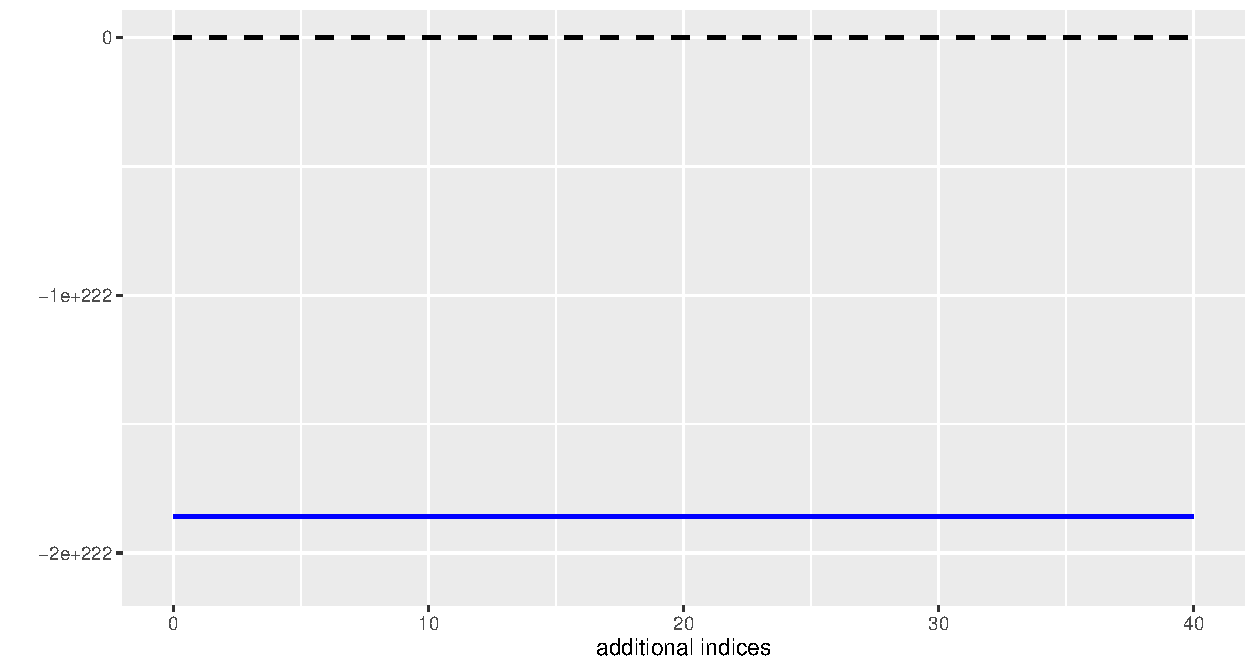
\includegraphics[scale=0.6]{plot100n.pdf}
\end{figure}
\end{frame}

% ---------------------------------------------------------------------------------------------------------------------------------------%


\begin{frame}{$r=-10$: rejection}
\begin{figure}
\centering
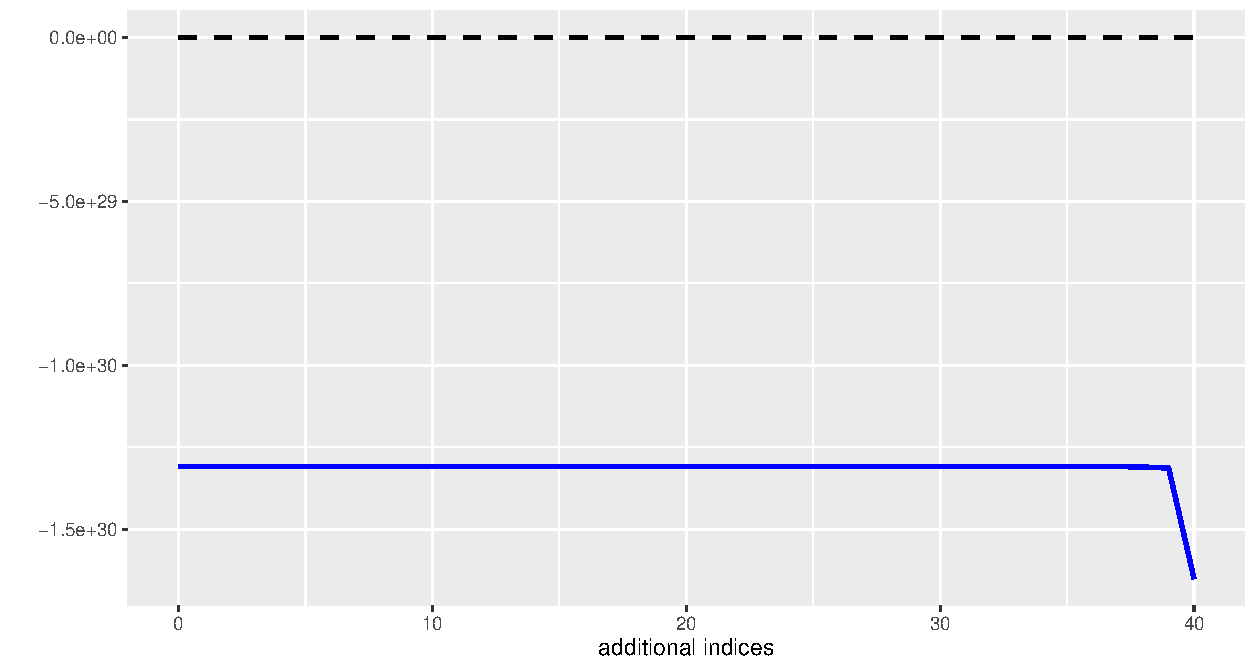
\includegraphics[scale=0.6]{plot10n.pdf}
\end{figure}
\end{frame}

% ---------------------------------------------------------------------------------------------------------------------------------------%

\begin{frame}{$r=-2$: rejection}
\begin{figure}
\centering
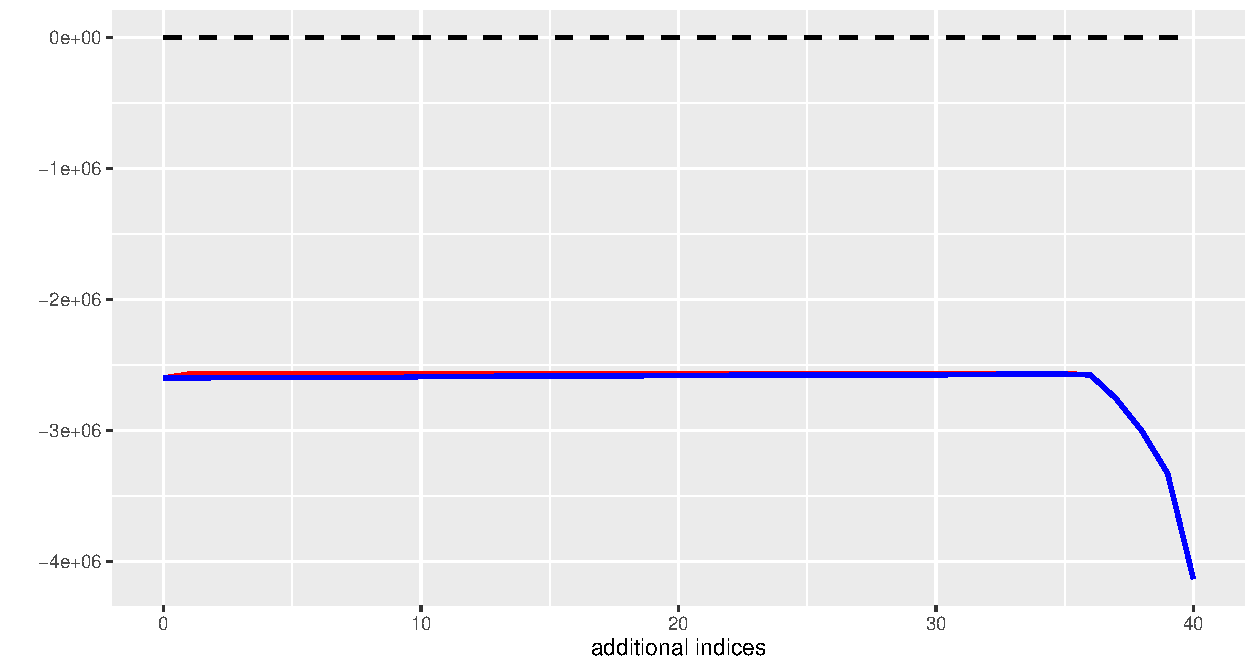
\includegraphics[scale=0.6]{plot2n.pdf}
\end{figure}
\end{frame}



% ---------------------------------------------------------------------------------------------------------------------------------------%


\begin{frame}{$r=-1$ (harmonic mean): rejection}
\begin{figure}
\centering
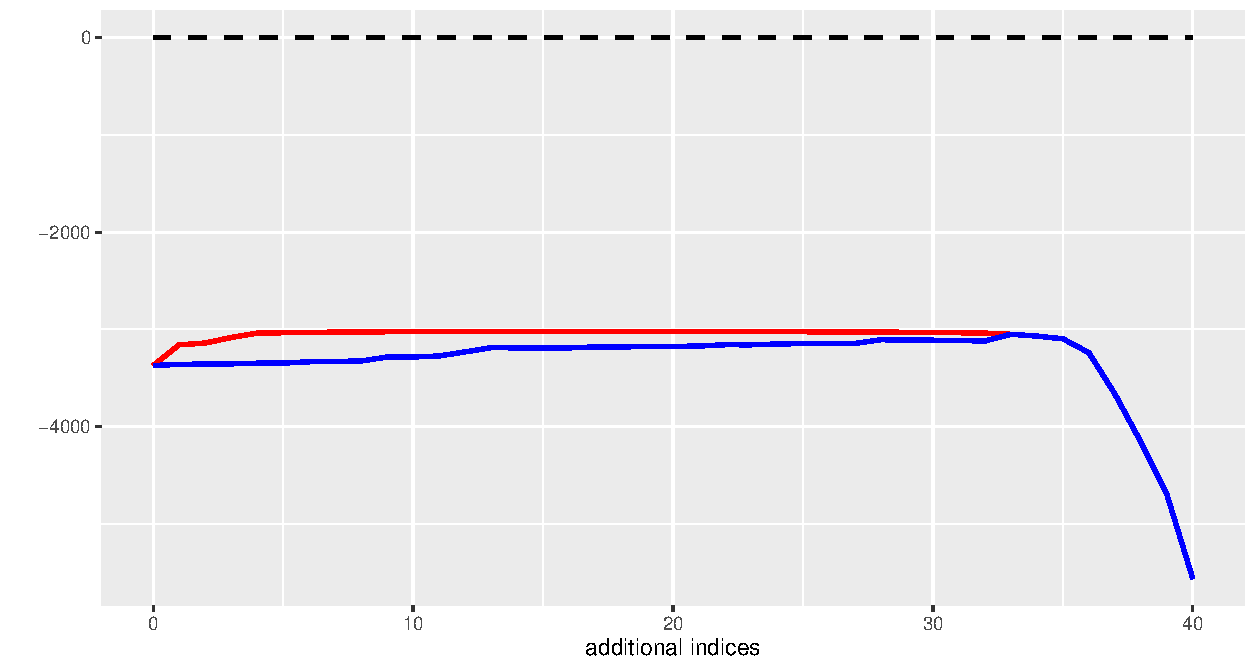
\includegraphics[scale=0.6]{plot1n.pdf}
\end{figure}
\end{frame}

% ---------------------------------------------------------------------------------------------------------------------------------------%


\begin{frame}{$r=-0.5$: rejection}
\begin{figure}
\centering
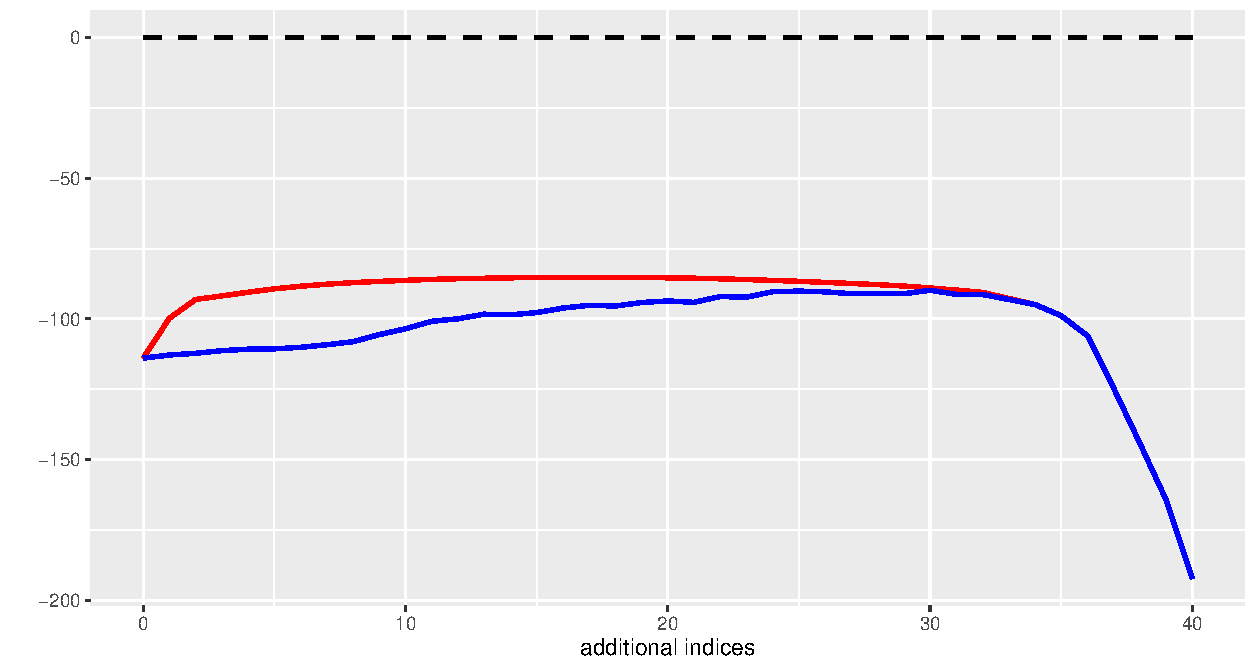
\includegraphics[scale=0.6]{plot05n.pdf}
\end{figure}
\end{frame}

% ---------------------------------------------------------------------------------------------------------------------------------------%


\begin{frame}{$r=-0.1$: rejection}
\begin{figure}
\centering
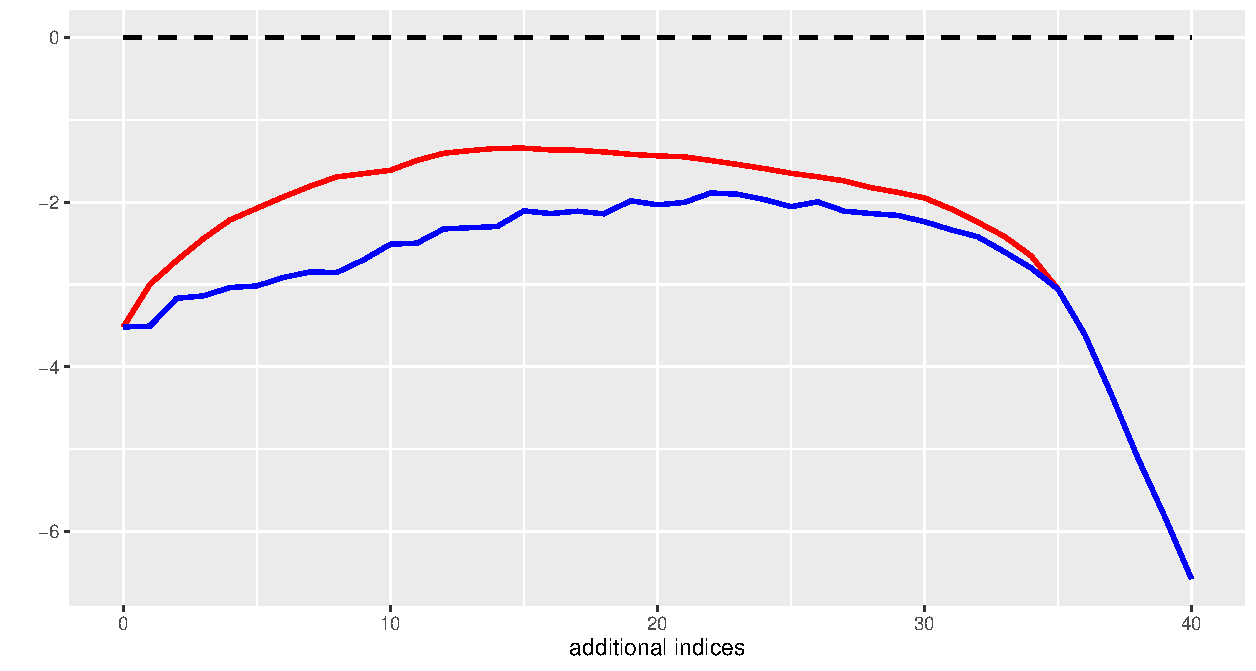
\includegraphics[scale=0.6]{plot01n.pdf}
\end{figure}
\end{frame}


% ---------------------------------------------------------------------------------------------------------------------------------------%


\begin{frame}{$r=0$ (geometric mean): rejection}
\begin{figure}
\centering
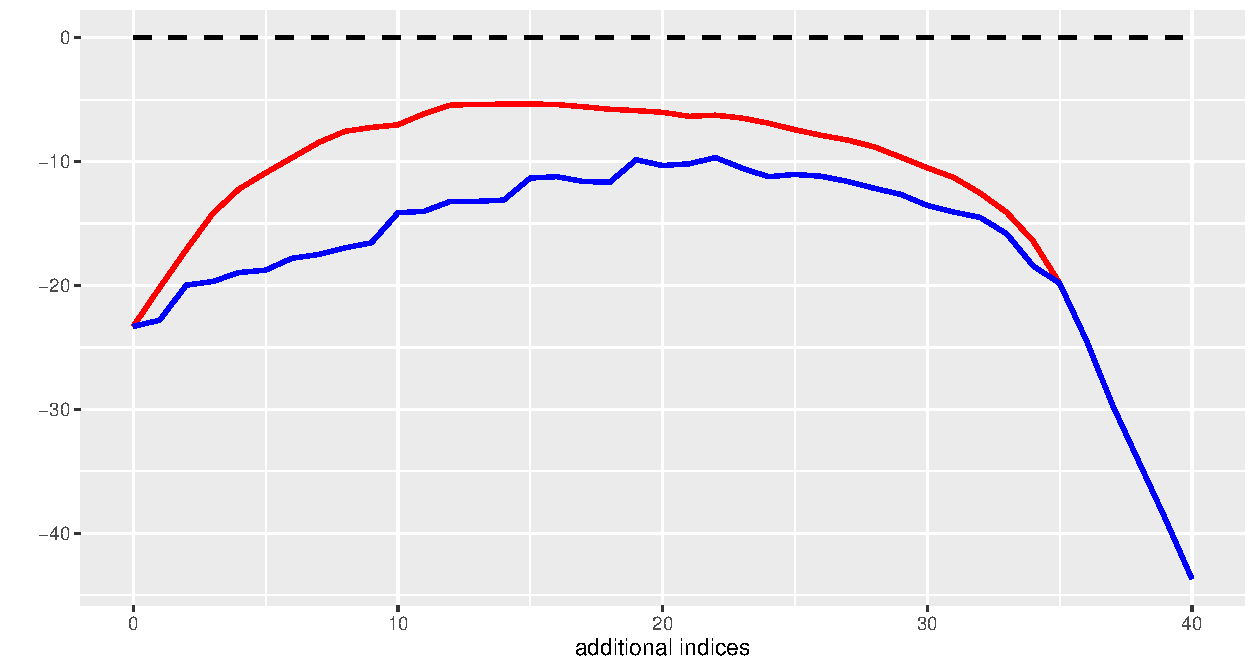
\includegraphics[scale=0.6]{plot0.pdf}
\end{figure}
\end{frame}

% ---------------------------------------------------------------------------------------------------------------------------------------%


\begin{frame}{$r=0.1$: rejection}
\begin{figure}
\centering
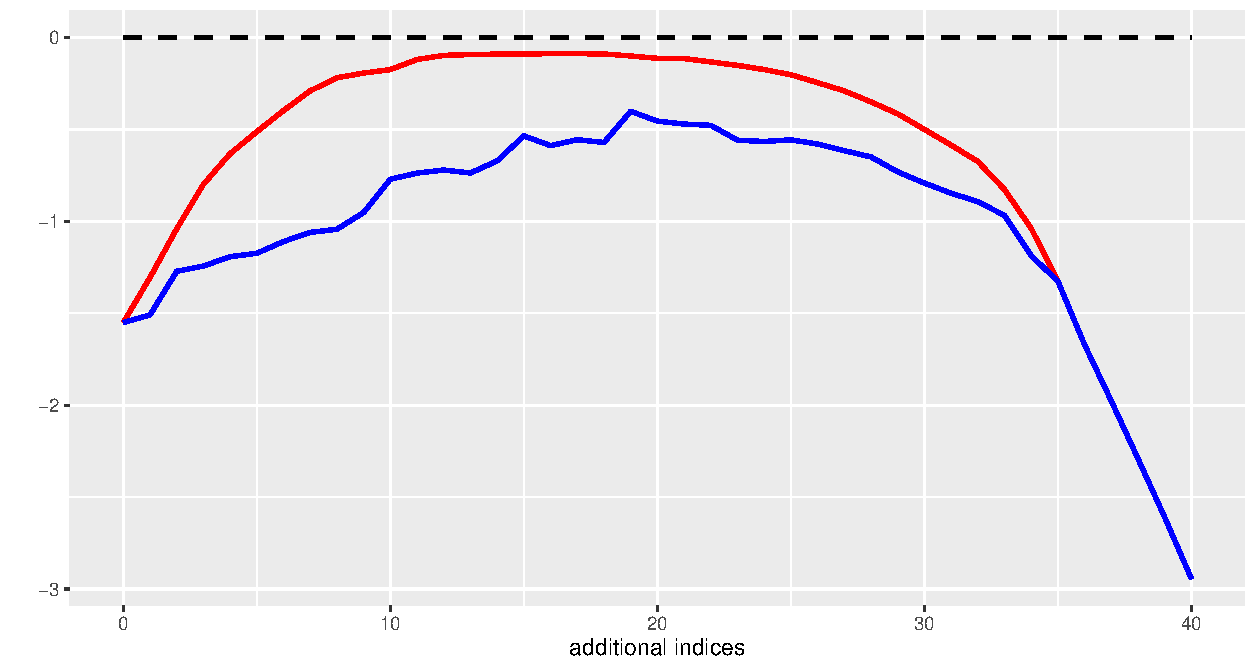
\includegraphics[scale=0.6]{plot01.pdf}
\end{figure}
\end{frame}

% ---------------------------------------------------------------------------------------------------------------------------------------%


\begin{frame}{$r=0.5$: non-rejection}
\begin{figure}
\centering
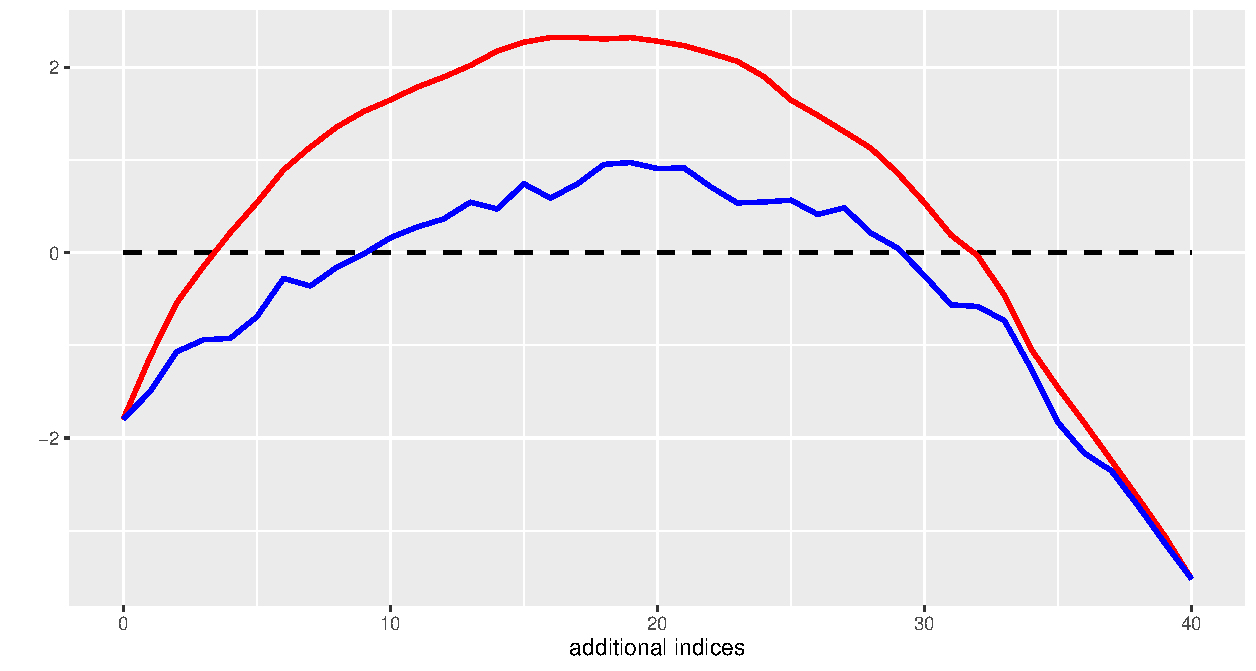
\includegraphics[scale=0.6]{plot05.pdf}
\end{figure}
\end{frame}

% ---------------------------------------------------------------------------------------------------------------------------------------%


\begin{frame}{$r=1$ (arithmetic mean): non-rejection}
\begin{figure}
\centering
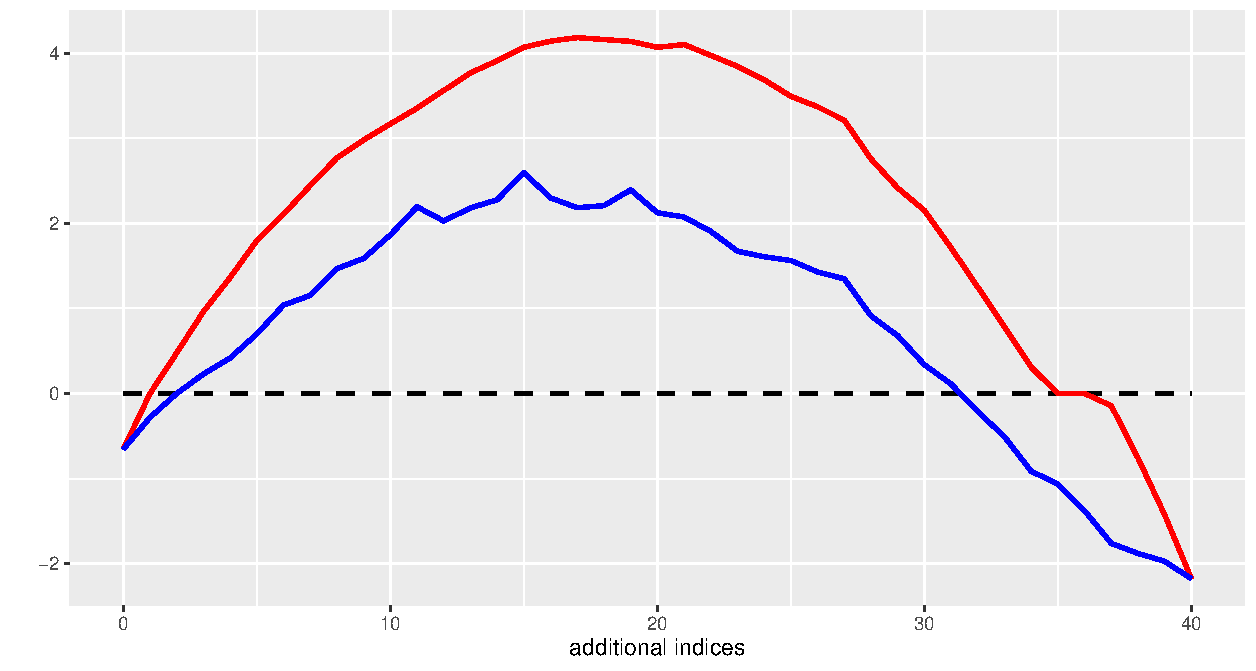
\includegraphics[scale=0.6]{plot1.pdf}
\end{figure}
\end{frame}

% ---------------------------------------------------------------------------------------------------------------------------------------%

\begin{frame}{$r=2$: non-rejection}
\begin{figure}
\centering
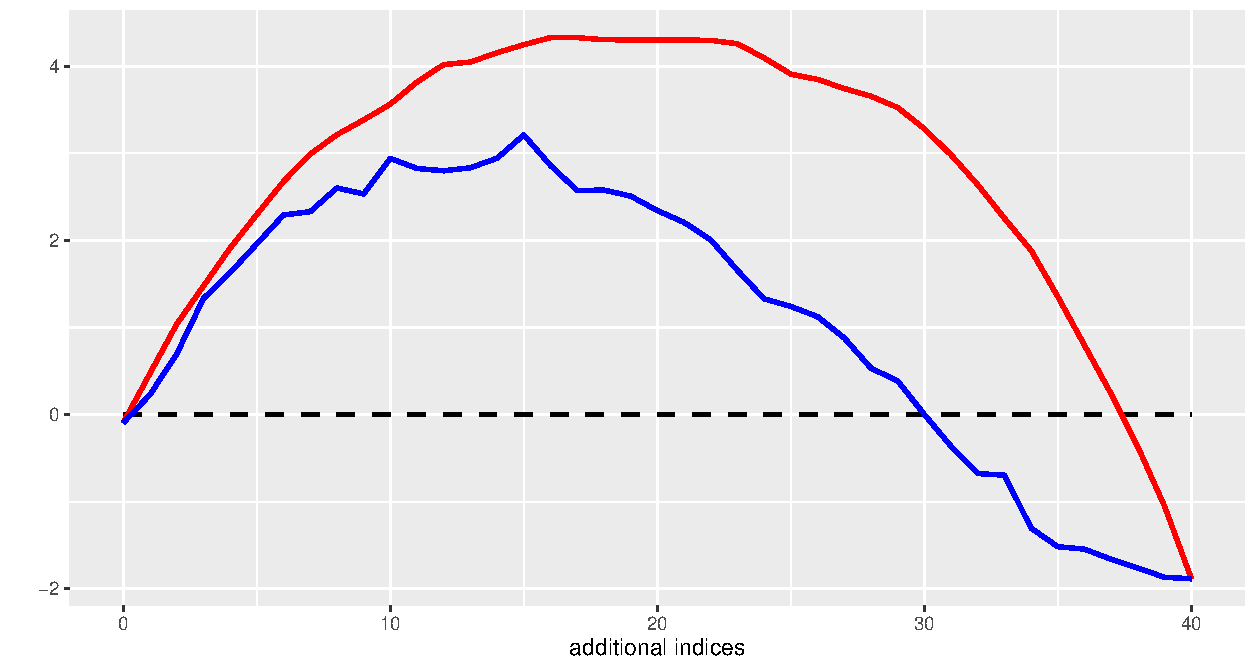
\includegraphics[scale=0.6]{plot2.pdf}
\end{figure}
\end{frame}

% ---------------------------------------------------------------------------------------------------------------------------------------%

\begin{frame}{$r=10$: non-rejection}
\begin{figure}
\centering
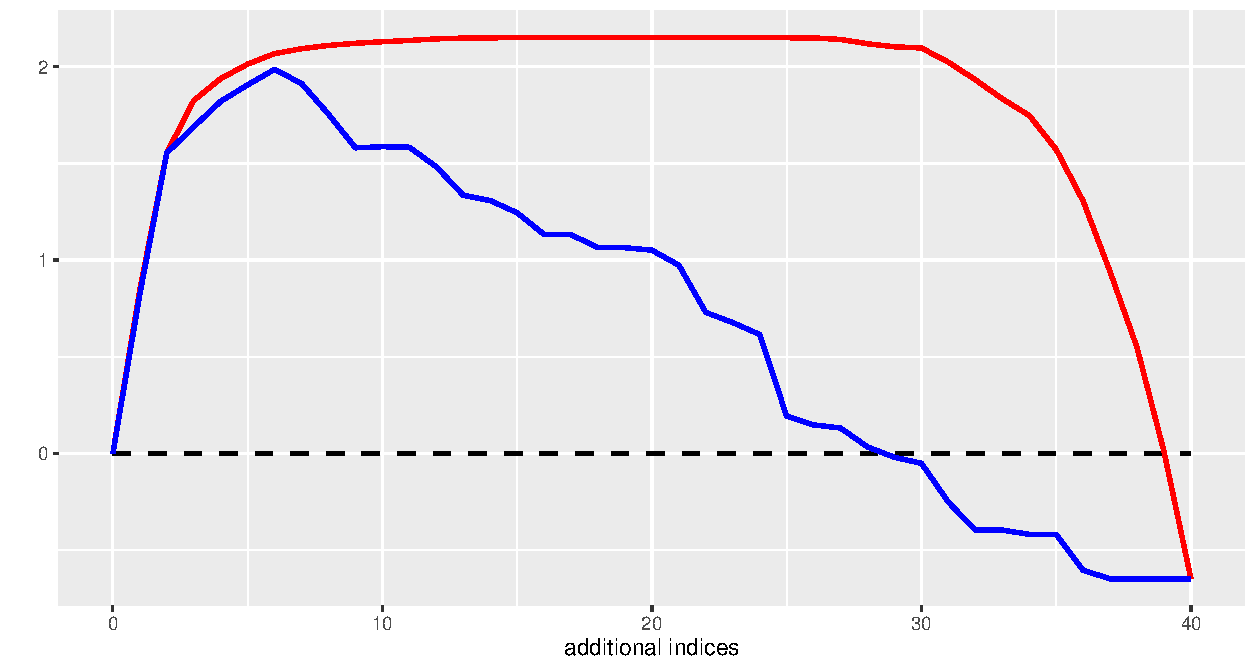
\includegraphics[scale=0.6]{plot10.pdf}
\end{figure}
\end{frame}

% ---------------------------------------------------------------------------------------------------------------------------------------%

\begin{frame}{$r=100$ ($\approx$ maximum): non-rejection}
\begin{figure}
\centering
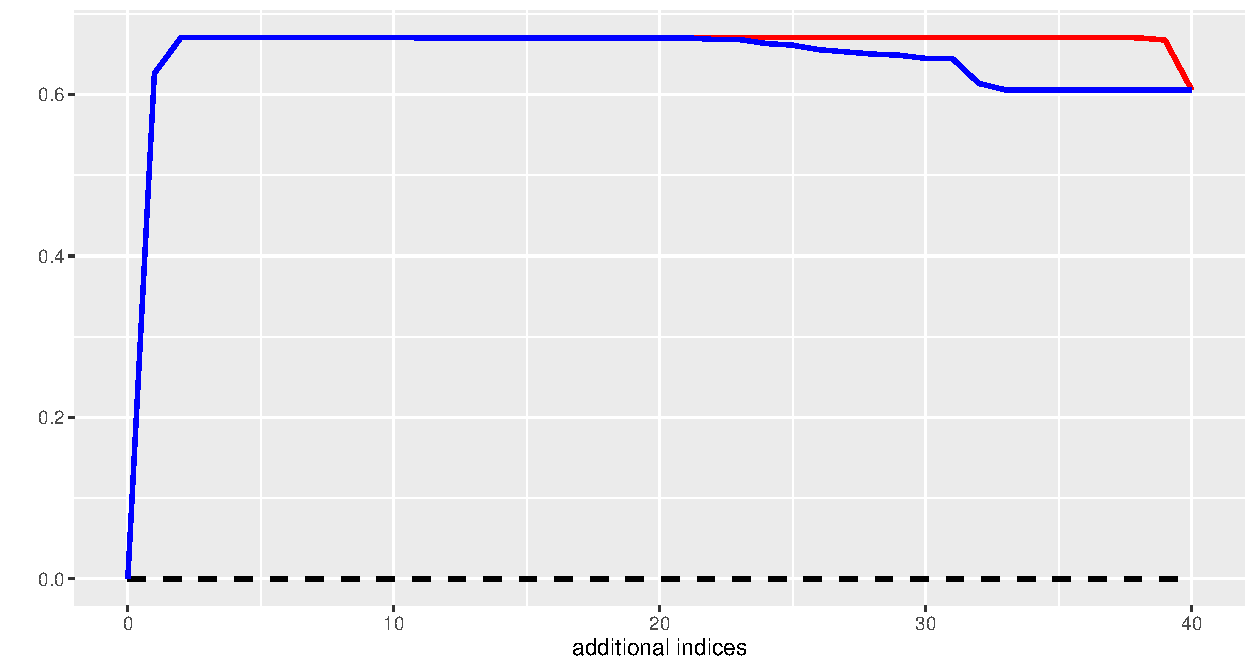
\includegraphics[scale=0.6]{plot100.pdf}
\end{figure}
\end{frame}


% ---------------------------------------------------------------------------------------------------------------------------------------%











%\section{Branch and Bound Iterations}

%\begin{frame}{Number of Iterations}
%The BAB was needed only in 18 cases out of 5733 ($0.3\%$), and only when $r\in[-1,2]$.

%\begin{table}[h!]
%\centering
%\resizebox{0.7\textwidth}{!}{
%\begin{tabular}{cccccccccc}
%\toprule
%$r$ & $s_{*}$ & $o_{*}$ & $s_{\text{size}}$ & $\rho$ & non-rej & RL & KL & RH & KH\\
%\midrule
%-2 & 10 & 80 & 20 & 0 & F & - & - & 106 & 106\\
%\midrule
%-1 & 0 & 0 & 80 & 0 & T & 337 & 27 & 8 & 97\\ 
%\midrule
%-0.1 & 20 & 80 & 20 & 0 & T & 606 & 328 & 146 & 1005\\
%\midrule
%\multirow{4}{*}{0}
% & 10 & 0 & 20 & 0 & F & - & - & 462 & 462\\
% & 10 & 50 & 50 & 0 & T & 560 & 34 & 153 & 154\\
% & 10 & 100 & 20 & 0.5 & F & 17 & 17 & 154 & 154\\
% & 20 & 100 & 20 & 0 & F & 58 & 58 & 176 & 176\\
%\bottomrule
%\end{tabular}
%}
%\end{table}
%\end{frame}


% ---------------------------------------------------------------------------------------------------------------------------------------%



%\begin{frame}{Number of Iterations}
%\begin{table}[h!]
%\centering
%\resizebox{0.7\textwidth}{!}{
%\begin{tabular}{cccccccccc}
%\toprule
%$r$ & $s_{*}$ & $o_{*}$ & $s_{\text{size}}$ & $\rho$ & non-rej & RL & KL & RH & KH\\
%\midrule
%\multirow{2}{*}{0.1}
% & 20 & 100 & 20 & 0 & T & 275 & 27 & 134 & 871\\
% & 50 & 50 & 20 & 0 & F & 186 & 186 & 280 & 280\\
%\midrule
%\multirow{2}{*}{0.5}
% & 20 & 20 & 80 & 0 & T & 41 & 17 & 14 & 34\\ 
% & 50 & 80 & 20 & 0.5 & F & 22 & 22 & 168 & 168\\
%\midrule
%\multirow{2}{*}{1}
% & 50 & 100 & 20 & 0 & F & 18 & 18 & 486 & 486\\
% & 80 & 80 & 20 & 0.5 & F & 28 & 28 & 210 & 210\\
%\midrule
%\multirow{4}{*}{2}
% & 50 & 50 & 80 & 0 & F & 16 & 16 & 42 & 42\\
% & 50 & 80 & 50 & 0 & F & 28 & 28 & 5716 & 5716\\
% & 80 & 100 & 20 & 0 & F & 12 & 12& - & -\\
% & 100 & 20 & 50 & 0 & T & 199 & 27 & 92 & - \\ 
%\bottomrule
%\end{tabular}
%}
%\end{table}
%\end{frame}







% ---------------------------------------------------------------------------------------------------------------------------------------%


%\begin{frame}{Number of Iterations}
%RH required the smallest number of iterations.

%\vspace{3mm}
%\begin{table}[h!]
%\centering
%\begin{tabular}{ccccc}
%\toprule
% & RL & KL & \textbf{RH} & KH\\
%\midrule
%$p$ & 22.2 & 27.8 & \textbf{72.2} & 38.9 \\
%$M$ & 3113 & 3072 & \textbf{1459} & 1822 \\
%\bottomrule
%\end{tabular}
%\end{table}

%\vspace{3mm}
%\begin{itemize}
%\item $p=$ percentage of simulations where the setting was optimal
%\item $M=$ mean of iterations (when the number exceeds the maximum, it is approximated to the maximum $10^4$)
%\end{itemize}
%\end{frame}







% ---------------------------------------------------------------------------------------------------------------------------------------%













\end{document}


%\begin{figure}
    %\centering
    %\includegraphics[scale=0.45]{estimate.pdf}
    %\label{fig:my_label}
%\end{figure}






